\chapter{Funciones}	

	\section{Función real de variable real}
	
		
Las funciones son las herramientas principales para la descripción matemática de una situación real. Todas las fórmulas de la Fí­sica no son más que funciones: expresan cómo ciertas magnitudes (por ejemplo el volumen de un gas) dependen de otras (la temperatura y la presión). El concepto de función es tan importante que muchas ramas de la matemática moderna se caracterizan por el tipo de funciones que estudian. No es de extrañar, por ello, que el concepto de función sea de una gran generalidad. Además, se trata de uno de esos conceptos cuyo contenido esencial es fácil de comprender aunque difí­cil de formalizar.

	En matemática, se dice que una magnitud es función de otra si el valor de la primera depende del valor de la segunda. Por ejemplo el área $A$ de un cí­rculo es función de su radio $r$ (el valor del área es proporcional al cuadrado del radio, $A = \pi\cdot r^2$). Del mismo modo, la duración $t$ de un viaje en tren entre dos ciudades separadas por una distancia $d$ de $150\;  km$ depende de la velocidad $v \; km/h$ a la que se desplace el tren (la duración $t$ es inversamente proporcional a la velocidad, $150 / v$). A la primera magnitud (el área, la duración) se la denomina \emph{variable dependiente}, y la magnitud de la que depende (el radio y la velocidad) es la \emph{variable independiente}.

	La palabra función fue introducida en Matemáticas por Leibniz, que utilizaba este término para designar cierto tipo de fórmulas matemáticas. Más tarde se vio que la idea de función de Leibniz tení­a un alcance muy reducido y, posteriormente, el significado de la palabra función fue experimentando generalizaciones progresivas. Actualmente, la definición de función es esencialmente la siguiente:
	
	\begin{defi}
		En análisis matemático, el concepto general de función, aplicación o mapeo se refiere a una regla que asigna a cada elemento de un primer conjunto $A$ (llamado \emph{Dominio o Campo de Existencia} de la función) un \underline{único elemento} de un segundo conjunto $B$ (llamado \emph{Recorrido o Rango} de la función).
		
		 Obsérvese que una función son tres cosas. el conjunto $A$ sobre el que actíúa la función, el conjunto $B$ en el que toma valores y la regla que la define. 
	
		 Esquemáticamente: $f: A \to B \; / \; \forall x \in A \leadsto \exists ! \; y=f(x) \in B$
		
	\end{defi}
	
		 En este curso nos van a interesar las \emph{funciones reales} ($B \in \mathbb R$) \emph{de variable real} ($A \in \mathbb R$).
	
	%\begin{figure}[H]
		%\centering
		%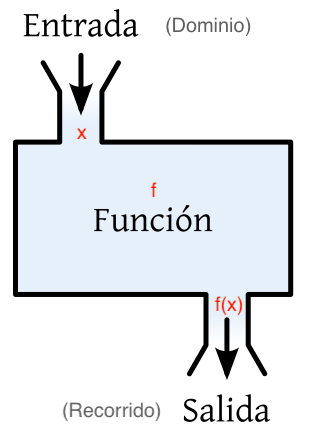
\includegraphics[width=0.3\textwidth]{imagenes/imagenes02/T02IM01.png}
		%\caption{Podemos considerar una función como una especie de máquina matemática que transforma unos números reales en otros.}
	%\end{figure}
	
	\begin{figure}[H]
		\centering
		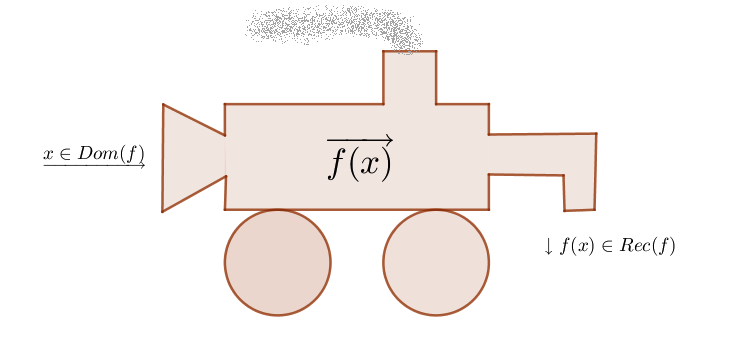
\includegraphics[width=0.7\textwidth]{imagenes/imagenes02/T02IM01b.png}
		\caption{Podemos considerar una función como una especie de máquina matemática que transforma unos números reales en otros.}
	\end{figure}
	

		
	 El dominio de una función puede restringirse según el contexto. Por ejemplo, el dominio de la función de área dado por $A = \pi r^2$ solamente permite que los radios $r$ sean positivos (ya que es una distancia). Cuando definimos una función $y =f(x)$ con una fórmula y el dominio no se da explí­citamente o está restringido por el contexto, se supone que es el máximo conjunto de valores de $x$ reales para los que la fórmula da valores reales de $y$; este dominio se llama dominio natural. Si queremos restringir el dominio de alguna manera, debemos especificarlo.
	\begin{multicols}{2}
	Los dominios naturales de las funciones polinómicas es $\mathbb R$, para las funciones racionales hay que excluir de $\mathbb R$ los números que anulen su denominador, las funciones radicales, de í­ndice par, el domino natural estará formado por todos los números $\mathbb R$ que hacen que el radicando sea no-negativo (desigualdad). Las funciones logarí­tmicas solo se pueden calcular si el argumento es positivo. Las tangentes no están definidas para múltiplos impares de $\pi/2$, etc.
	
		\begin{figure}[H]
			\centering
			\includegraphics[width=0.35
			\textwidth]{imagenes/imagenes02/xiste02.png}
		\end{figure}
		\end{multicols}
	 \begin{defi}
	Llamamos \emph{gráfica} de una función $f$ a los puntos del plano $(x,y)$ tales que $y=f(x)$. Más concretamente:
	
	$G(f)=\{ (x,y)\in 	\mathbb R^2 \; / \; x\in Dom(f) \wedge y=f(x) \in Rec(f)   \}$	
	\end{defi}
	
	 La gráfica de una función nos da mucha información. A partir de la gráfica podemos saber:
	
	\begin{itemize}
		\item \emph{$Dom(f)$} se puede obtener sin más que ``proyectar'' la función sobre el eje $OX$. La zona sombreada constituye el dominio de la misma. (En rojo en la figura \ref{fig:dom-rec})
		\item \emph{$Rec(f)$} se puede obtener sin más que ``proyectar'' la función sobre el eje $OY$. La zona sombreada constituye el recorrido de la misma. (En verde en la figura \ref{fig:dom-rec})

		\item \emph{Estrategia de la vertical:} sabemos que una curva es la gráfica de una función matemática si al trazar lí­neas verticales, éstas cortan ninguna o \underline{una sola vez} a la curva. (Lí­neas grises en la figura \ref{fig:dom-rec})
		
	\end{itemize}

	\begin{figure}[H]
		\centering
		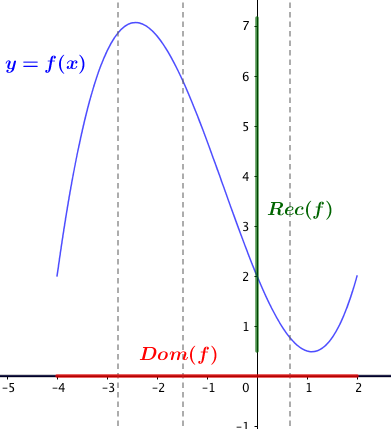
\includegraphics[width=0.5\textwidth]{imagenes/imagenes02/T02IM02.png}
		\caption{Gráfica de una función (azul), con su dominio (rojo) y recorrido (verde). Las lí­neas grises son la prueba de la vertical que asegura que $f$ es una función.}
		\label{fig:dom-rec}
	\end{figure}
		
	\begin{defi}[Igualdad de funciones]. 
	
	$f=g$ cuando $Dom(f)=Dom(g)\; $ y $\; f(x)=g(x),; \forall x\; $ en el dominio común.
		
	\end{defi}
		
	Es decir, dos funciones con la misma regla que las defina (fórmula) pero que tengan dominios diferentes se consideran funciones distintas.	
		
	
	\section{Operaciones con funciones}
		
		\begin{defi}{Funciones Elementales}
		
		En matemáticas, una \emph{función elemental} es una función construida a partir de una cantidad finita de funciones elementales fundamentales y constantes mediante operaciones racionales (adición, sustracción, multiplicación y división) y la composición de funciones usando exponenciales, logarí­tmicas, potenciales, constantes y las funciones trigonométricas y sus inversas, todas consideradas dentro del grupo de funciones elementales fundamentales.
			
		\end{defi}
		
		 Son \emph{funciones elementales fundamentales}:
		
		\begin{enumerate}
			\item Función constante: $f(x)=c,\; c\in \mathbb R$
			\item Función identidad: $f(x)=x$
			\item Función potencial: $f(x)=x^k,\; k\in \mathbb R \sim \{0\}$. Este tipo de funciones comprende a la función cuadrática $x^2$, la cúbica $x^3$, la raí­z $\sqrt x = x^{1/2}$, etc.
			\item Función exponencial: $f(x)=a^x,\; x\in \mathbb R,\; a\in \mathbb R^+ \sim \{ 1 \}$
			\item Función logarí­tmica: $f(x)=\log_a (x),\; x\in \mathbb R^+ ,\; a\in \mathbb R^+ \sim \{ 1 \}$
			\item Funciones trigonométricas: $f(x)=\sin x\; ; \quad f(x)=\cos x\; ; \qquad f(x)=\tan x \;  (x\neq (2k+1) \cdot 	\frac {\pi} {2}, \; k\in \mathbb Z)$
			\item Funciones trigonométricas inversas: $f(x)=\arcsin (x)\; (x\in [-1,1]); \quad f(x)=\arccos (x)\; (x\in [-1,1]); \quad f(x)=\arctan (x)\; (\forall x \in \mathbb R) $
		\end{enumerate}
		
		\begin{defi}{Suma, producto y cociente de funciones}.
			
			
			Dadas $f,g: A \to \mathbb R$, se define:
			
			\begin{itemize}
				\item producto por un número: $(kf)(x)=k\cdot f(x),\; k\in \mathbb R$, se representa por $kf$
				\item suma: $(f+g)(x)=f(x)+g(x)$, se representa por $f+g$
				\item producto: $(f\cdot g)(x)=f(x)\cdot g(x)$, se representa por $fg$
				\item cociente: $(f/g)(x)=f(x)/g(x),\; x\in A\; / \; g(x)\neq 0$, se representa por $f/g$
			\end{itemize}
			
		\end{defi}
		
		Obviamente un número se puede multiplicar por uno dado si existe el primero, dos números se pueden sumar, restar o multiplicar si ambos existen y, por último, dos números se pueden dividir si, existiendo ambos, el divisor es distinto de cero. Es por ello que:
		
		$Dom(k\cdot f)=Dom(f); \quad Dom(f+g)=Dom(f-g)=Dom(f\cdot g)=Dom(f) \cap Dom(g); \quad Dom(f/g)=Dom(f) \cap Dom(g)\sim \{x/g(x)=0 \}$

	\begin{prop} $\forall \; f,g,h : A \to \mathbb R\; $ se verifican las siguientes propiedades:
	
		\begin{enumerate}
			\item Asociativas: $(f+g)+h=f+(g+h); \qquad (fg)h=f(gh) $
			\item Conmutativas: $f+g=g+f; \qquad fg=gf$
			\item Distributiva: $(f+g)h=fh+gh$
		\end{enumerate}
	\end{prop}
	\begin{proof} La demostración es inmediata pues se reduce a las propiedades de los números reales.	
	\end{proof}

	\subsection{Composición de funciones y función inversa}
	
	

	\begin{defi}{Composición de funciones}.
	
	Sean $f:A \to \mathbb R, \; g:B \to \mathbb R$, tales que $f(A) \subset B$. En este caso, la función $h:A \to \mathbb R$ dada por $h(x)=g \left( f(x) \right)$ se llama \emph{composición de $g$ con $f$} y se representa por $h=g \circ f$. Es importante observar que la composición $h=g \circ f$ está definida solo si la imagen de $f$ está contenida en el dominio de $g$.
	
	
	La composición de funciones es asociativa, pero no-conmutativa.
	
	
	\begin{itemize}
		\item Asociativa: $(f \circ g) \circ h =f \circ (g \circ h) $
		\item No-Conmutativa: $f \circ g \neq g \circ f$
	\end{itemize}
		
	\end{defi}
	
	\begin{figure}[H]
		\centering
		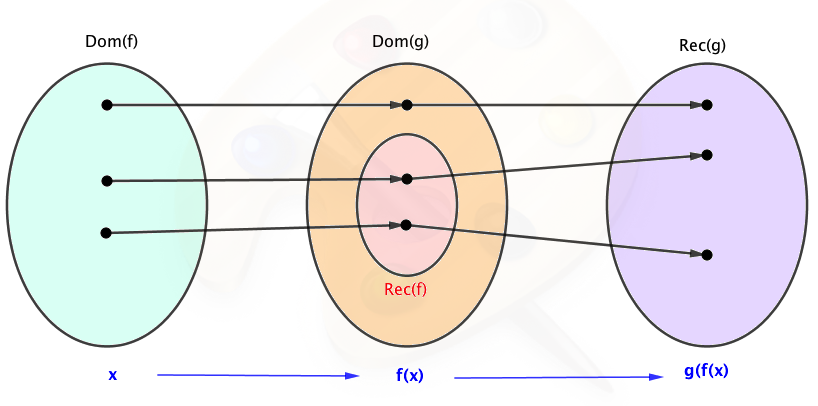
\includegraphics[width=0.6\textwidth]{imagenes/imagenes02/T02IM03.png}
		\caption{Composición de funciones.}
	\end{figure}
		

		\begin{defi}{Funciones Inyectivas}.
		
		 Se dice que $f:A\to \mathbb R$ es \emph{inyectiva} en un conjunto $C \subset A$ si en puntos distintos de $C$ toma valores distintos, es decir, si $\forall x,y \in C,\; x\neq y \to f(x) \neq f(y)$ 	
	
		\end{defi}
		\emph{Prueba de la lí­nea horizontal}. Dada la gráfica de una función, si al trazar lí­neas horizontales, paralelas al eje $OX$ cortamos más de una vez a la función, entonces no será inyectiva.
		
		\begin{figure}[H]
			\centering
			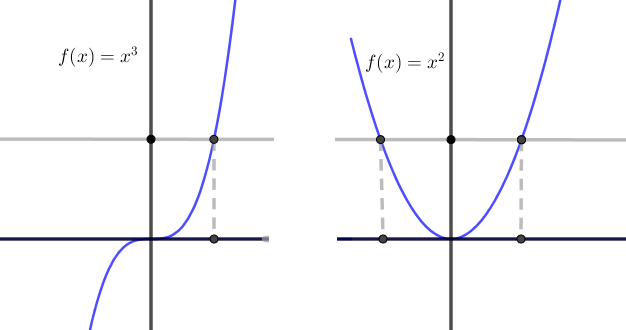
\includegraphics[width=0.6\textwidth]{imagenes/imagenes02/T02IM04.png}
			\caption{Prueba de la lí­nea horizontal: la primera función sí­ es inyectiva y la segunda no, la lí­nea horizontal corta más de una vez a la gráfica.}
		\end{figure}
		
		La importancia de la inyectividad está en que cuando resolvamos ecuaciones basadas en funciones inyectivas, la solución será única ($f(x)=x^2$ no es inyectiva, al resolver $x^2=4 \to x=|2|=\pm 2$, en cambio, $g(x)=x^3$ sí­ es inyectiva, por ello, $\sqrt [3] {-8}=-2$, tiene solución única). También es importante la inyectividad de una función a la hora de calcular su función inversa, como veremos a continuación.
		
		\begin{defi} {Función inversa} (de una función inyectiva).
		
		
			Si $f:A \to \mathbb R$ es una \emph{función inyectiva}, puede definirse una nueva función $f^{-1}:B=f(A) \to 	\mathbb R$, que llamaremos \emph{función inversa} de $f$, que $\forall y\in B=f(A), \; \exists ! x\in A: \; f(x)=y$. Equivalentemente, $f^{-1} \left(  f(x) \right)=x, \; \forall x \in A$ y también $f \left( f^{-1}(y)  \right) = y,\; \forall y \in B=f(A)$.

		\end{defi}
		
		Para calcular la inversa de una función (lo veremos en los ejercicios resueltos) escribiremos $y=f(x)$, cambiaremos las $x$ por las $y$ y, por último, despejaremos la $y=f^{-1}(x).$
		
		 Considerando una función (inyectiva) como una máquina que transforma unos números en otros, la función inversa serí­a como conectar la máquina al revés. Todo ello hace que se intercambien los papeles $x\leftrightarrow y$. En la gráfica de la función identidad $y=f(x)=x$ es en la que tanto $x$ como $y$ juegan el mismo papel, por ello \emph{las gráficas de $f$ y $f^{-1}$} serán \emph{simétricas} respecto de la bisectriz del primer y tercer cuadrante ( que es la gráfica de la función identidad $y=f(x)=x=I(x)\,)$.
		
		
		
		\begin{prop}{Propiedades de la función inversa.}
		\label{prop:funcion-inversa}
		\begin{itemize}
			
			\item $Dom(f^{-1})=Rec(f); \quad Rec(f^{-1})=Dom(f)$
			\item $ \left( f^{-1} \right) ^{-1} (x)=f(x) $
			\item $ (f \circ f^{-1}) (x)= I(x)=x; \quad (f \circ f^{-1})(x)=I(x)=x$
			\item $ \left( f \circ g   \right)^{-1}(x)=\left(  g^{-1}\circ f^{-1} \right)(x) $	
			
			\footnotesize{Esta última curiosa propiedad es caracterí­stica de las operaciones no conmutativas, en el producto de matrices (invertibles), que es no conmutativo, también se da de forma similar: $(A\cdot B)^{-1}=B^{-1}\cdot  A^{-1}$}
		\end{itemize}	
		
		\end{prop}
		
		\begin{proof}
			La demostración de estas propiedades algebraicas de la función inversa es la aplicación directa de la definición.
		\end{proof}
		
		\emph{Nota:} No hay que confundir \emph{función inversa} $f^{-1}(x)$, que es cuando la función `marcha al revés'  con la \emph{inversa de una función} que es $\dfrac 1 {f(x)}$.
		

		\begin{figure}[H]
			\centering
			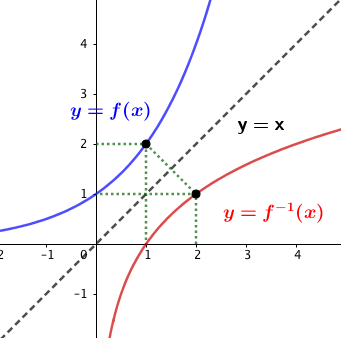
\includegraphics[width=0.3\textwidth]{imagenes/imagenes02/T02IM05.png}
			\caption{Gráficas de una función y su función inversas, simétricas respecto de $y=x$.}
		\end{figure}
		
		\textbf{Funciones arco.}
		
		 La función $y=\sin x$ es no-inyectiva, pero si nos quedamos con un tramo en que sí­ lo es, $[-\pi/2, \pi/2]  \; \;  \underrightarrow { \sin x } \; \;  [-1,1]$ podemos tomar su función inversa: $y=\arcsin x: [-1,1] \to [-\pi/2, \pi/2] $
		
		Se verifica que $\quad \sin (\arcsin x)=x; \qquad \arcsin (\sin x)=x$
		
		 Lo mismo para la función $y=\cos x$ es no-inyectiva, pero si nos quedamos con un tramo en que sí­ lo es, $[0, \pi]  \; \;  \underrightarrow { \cos x } \; \;  [-1,1]$ podemos tomar su función inversa: $y=\arccos x: [-1,1] \to [0, \pi] $
		
		Se verifica que $\quad \cos (\arccos x)=x; \qquad \arccos (\cos x)=x$
		
		
		
		\begin{figure}[H]
			\centering
			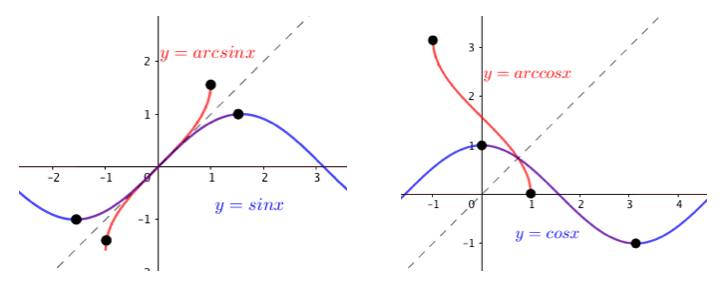
\includegraphics[width=0.8\textwidth]{imagenes/imagenes02/T02IM06.png}
			\caption{Funciones arco: arco seno y arco coseno y zonas de inyectividad de seno y coseno..}
		\end{figure}
		
		La función tangente es periódica, de periodo $\pi$. Tomando uno de estos periodos en que la tangente es inyectiva: $[-\pi/2, \pi/2] \; \;  \underrightarrow { \tan x } \; \; \mathbb R $, podemos tomar su función inversa: $y=\arctan x: \mathbb R \to [-\pi/2, \pi/2]$
		
		Se verifica que $\quad \tan (\arctan x)=x; \qquad \arctan (\tan x)=x$
		
		
		\begin{figure}[H]
			\centering
			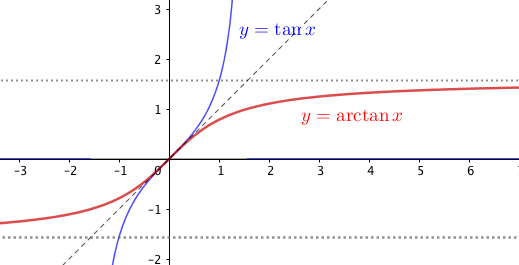
\includegraphics[width=0.6\textwidth]{imagenes/imagenes02/T02IM07.png}
			\caption{Función arco tangente.}
		\end{figure}
		
		

		
		\section{Transformaciones elementales de funciones}
		\subsection{Traslaciones}
		\begin{itemize}
			\item Traslaciones Verticales: $y=f(x)+k$
			
			Desplaza a la función $f(x)$ $k$ unidades hacia arriba si $k>0$ o hacia abajo si $k<0$
			
			\item Traslaciones Horizontales: $y=f(x+h)$
			
			Desplaza a la función $f(x)$ $h$ unidades hacia la izquierda si $h>0$ o hacia la derecha si $h<0$
		\end{itemize}
		
		\begin{figure}[H]
			\centering
			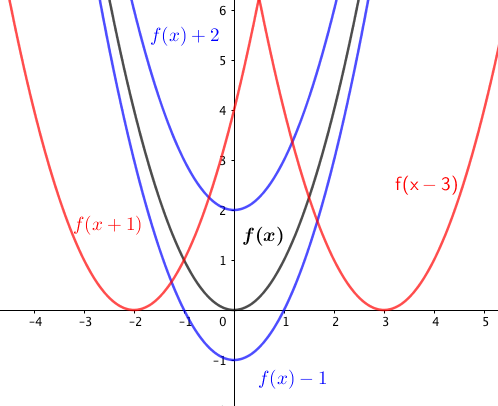
\includegraphics[width=0.4\textwidth]{imagenes/imagenes02/T02IM08.png}
			\caption{Traslaciones.}
		\end{figure}
		
		\subsection{Simetrí­as}
		
		\begin{itemize}
			\item $y=-f(x)$: Simetriza a la función respecto del eje $OX$
			\item $y=f(-x)$: Simetriza a la función respecto del eje $OY$
		\end{itemize}
		
		\begin{figure}[H]
			\centering
			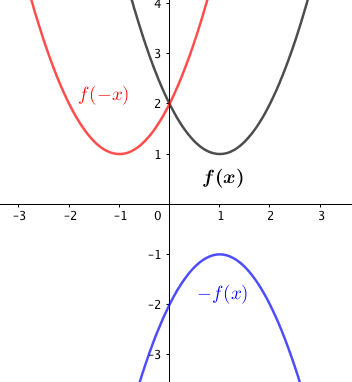
\includegraphics[width=0.3\textwidth]{imagenes/imagenes02/T02IM09.png}
			\caption{Simetrí­as.}
		\end{figure}
		
			\begin{defi} Paridad de una función.
			
			 Dada $f(x)$, calculamos $f(-x)$ y pueden pasar tres cosas:	
			
			\begin{itemize}
				\item [-] $f(-x)=f(x) \to $ función PAR, simétrica respecto de $OY$
				\item [-] $f(-x)=-f(x) \to $ función IMPAR, simétrica respecto de $OX$
				\item [-] Otra cosa $\to$ función sin paridad.
			\end{itemize}
			\end{defi}
			
		\begin{figure}[H]
		\centering
		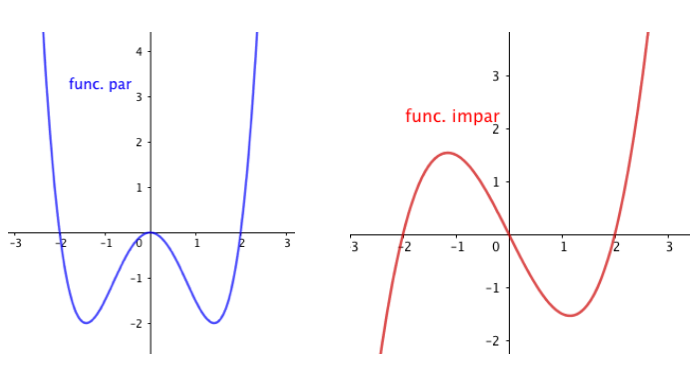
\includegraphics[width=0.5\textwidth]{imagenes/imagenes02/T02IM10.png}
		\caption{Paridad.}
		\end{figure}
		

		\subsection{Estiramientos y contracciones}
		\begin{itemize}
			\item Verticales: $y=b f(x)$. Para $b>1$ se produce un estiramiento vertical, para $0<b<1$ una contracción vertical.
			\item Horizontales: $y=f(ck)$. Para c>1 se produce un estiramiento horizontal, para $0<c<1$ una contracción horizontal.
		\end{itemize}
		
		\begin{figure}[H]
			\centering
			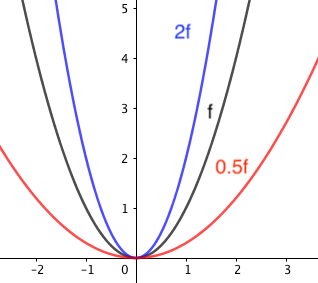
\includegraphics[width=0.3\textwidth]{imagenes/imagenes02/T02IM11.png}
			\caption{Estiramientos y contracciones verticales.}
		\end{figure}
		
		\subsection{Funciones monotónas, acotadas y periódicas}
		
		\begin{defi}Funciones monótonas.
		
		 Se dice que $f:A \to \mathbb R$ es monótona creciente (decreciente) en un conjunto $C\subset A$ si $\forall x_1, x_2 \in C$ con $x_1\le x_2$, entonces $f(x_1)\le f(x_2)$. ($f(x_1)\ge f(x_2)$, para decreciente).
		\end{defi}
		
		\begin{defi} Funciones acotadas.
		
		Una función $f(x)$ está acotada en un conjunto $A$ si existe un número real $K$ tal que $|f(x)|\le K,\; \forall x \in A$	
		
		Si no se especifica el conjunto $A$ se supone que es todo su $Dom(f)$ y, en tal caso, la gráfica de $f$ estará contenida en una banda horizontal definida por las rectas $y=k$ e $y=-k$
		
		\end{defi}
		
		\begin{defi} Funciones periódicas.
		
		Una función es periódica	 si existe un número real $T\neq 0$ tal que $f(x+T)=f(x)$. A este número $T$ se le llama periodo.
		
		Las funciones $\sin x$ y $\cos x$ son periódicas de periodo $2\pi$. La función $\tan x$ tiene periodo $\pi$.
		\end{defi}

		\begin{figure}[H]
			\centering
			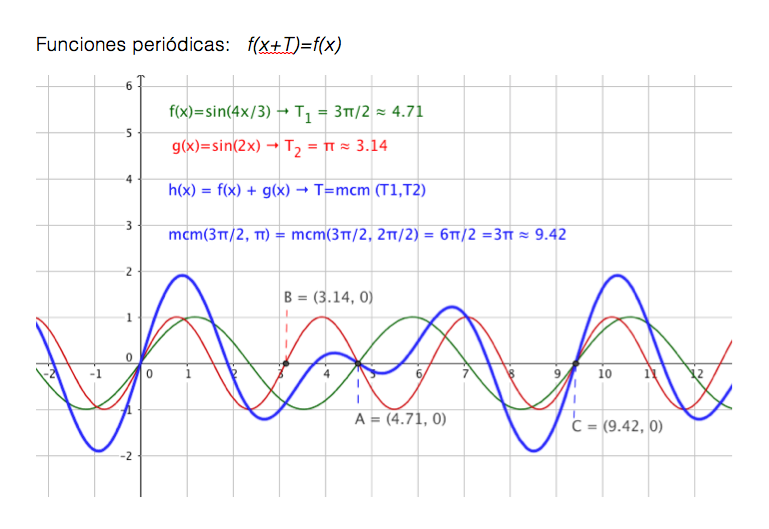
\includegraphics[width=0.6\textwidth]{imagenes/imagenes02/T02IM25.png}
			\caption{$\divideontimes$ Función periódica}
					\end{figure}
		
		\section{Otro tipo de funciones}
		
		\subsection{Funciones definidas a trozos}
		
		\begin{defi}{Función definida a trozos}.
		
		$f: A \to B$. Supongamos que A puede representarse como una unión de conjuntos disjuntos, con $A_i: \; A=\bigcup_{i=1}^{n}{{A}_{i}} $, entonces f es una \underline{función definida a trozos} si $\forall x \in A_i:\; f(x)=f_i(x),\; 1\le x \le n$
			
		\end{defi}

		
		 La función más famosa que ya vimos en el capí­tulo anterior fue el valor absoluto:
		
		\begin{equation*}
		|x|=
		\begin{cases} 
		\;\;  x &\mbox{if } x\ge 0 \\ 
		\; -x & \mbox{if } x<0 
		\end{cases}
		\end{equation*}
	
		 Otras funciones interesantes y también definidas a trozos son la \emph{parte entera} y la \emph{parte decimal} o mantisa de un número real, definidas como:
		 
		 Parte entera: $\left\lfloor x \right\rfloor = $ entero anterior o igual a x.
		 
		 Parte decimal: $Dec(x)=x-\left\lfloor x \right\rfloor$
		 
		 Vemos sus gráficas en la siguiente imagen.
		 
		\begin{figure}[H]
			\centering
			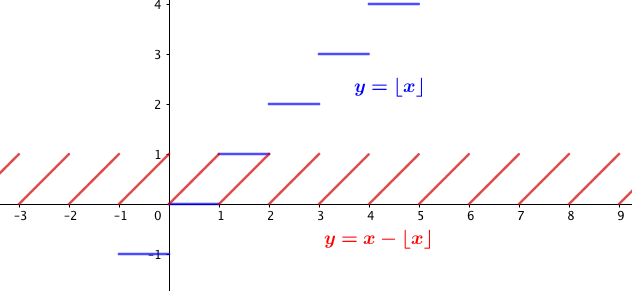
\includegraphics[width=0.7\textwidth]{imagenes/imagenes02/T02IM12.png}
			\caption{Funciones parte entera y parte decimal}
		\end{figure}
		
		 \begin{multicols}{2}
		 Otra función definida a trozos que merece especial interés es la \emph{función de Dirichlet}
		
		\begin{equation*}
		f(x)=
		\begin{cases} 
		\;\;  0 &\mbox{if } x \in \mathbb{Q} \\ 
		\; 1 & \mbox{if } x \in \mathbb{R} \sim \mathbb{Q} 
		\end{cases}
		\end{equation*}
		
		\begin{figure}[H]
			\centering
			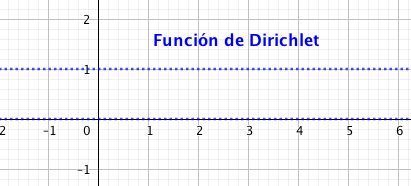
\includegraphics[width=0.4\textwidth]{imagenes/imagenes02/T02IM13.png}
			\caption{Función de Dirichlet (`discontinua' en todo su dominio).}
			\label{fig:dirichlet}
		\end{figure}
		\end{multicols}
		
		\subsection{Funciones hiperbólicas $\; \divideontimes$ }
		\label{subsec:func-hiperb}
		
		$\sinh (x)= \dfrac {e^x-e^{-x}}{2}; \qquad \cosh (x)= \dfrac {e^x+e^{-x}}{2}; \qquad \tanh (x)= \dfrac {e^x-e^{-x}}{e^x+e^{-x}}$
		
		\begin{prop} Las funciones hiperbólicas cumplen las siguientes propiedades:
		
		\begin{itemize}
			\item $\dfrac {\sinh (x)}{\cosh (x)}= \tanh (x)$
			\item $\cosh^2(x)-\sinh^2(x)=1 $
			\item $\sinh(x+y)=\sinh(x)\; \cosh (y) \; + \; \cosh(x) \; \sinh(x)$
			\item $\cosh(x+y)=\cosh(x)\; \cosh (y) \; - \; \sinh(x) \; \sinh(x)$
			%\item $(\sinh(x))'=\cosh(x); \qquad (\cosh(x))'=\sinh(x); \qquad (\tanh(x))'=\dfrac 1 {\cosh^2(x)}$
			\item El seno hiperbólico ($\sinh(x)$) y la tangente hiperbólica ($\tanh(x)$) son funciones \emph{impares}, el cosenos hiperbólico ($\cosh(x)$) es \emph{par}.
		\end{itemize}
			
		\end{prop}
		
		\begin{proof}
			La demostración es evidente a partir de las definiciones de las funciones hiperbólicas, por lo que se deja como ejercicio.
		\end{proof}

		\begin{figure}[H]
			\centering
			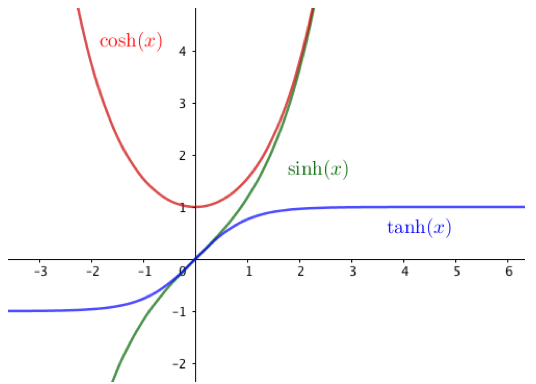
\includegraphics[width=0.5\textwidth]{imagenes/imagenes02/T02IM14.png}
			\caption{Funciones hiperbólicas.}
		\end{figure}
		
		 \small{La curva en paramétricas $x=\cosh (t);\; y=\sinh(t)$ verifica que $x^2-y^2=\cosh^2 (t)-\sinh^2(t)=1$, que corresponde a una \emph{hipérbola equilátera, por ello lo de funciones hiperbólicas. La curva en paramétricas $x=\cos (t);\; y=\sin(t)$  cumple que $x^2+y^2=1$, por ello al seno y coseno se les llaman funciones circulares.}
		
		
		\subsection{Función logí­stica  $\; \divideontimes$}
		
		Las poblaciones de seres vivos comienzan creciendo según la curva exponencial, pero con el tiempo llegan a invadir su espacio vital y su crecimiento se va amortiguando. La curva tí­pica de esta situación es la que se muestra en la siguiente figura.
		
		\begin{figure}[H]
			\centering
			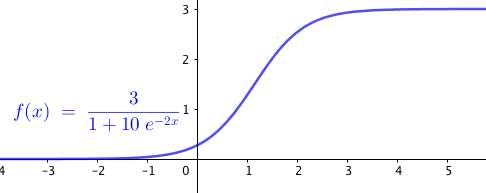
\includegraphics[width=0.4\textwidth]{imagenes/imagenes02/T02IM15.png}
			\caption{Función logí­stica.}
		\end{figure}
		
		 Función logí­stica: $f(x)=\dfrac {l}{1+ke^{-ax}}$
		
		\begin{itemize}
			\item [*] $l$ es la población lí­mite.
			\item [*] $1/(1+k)$ es la población con $x=0$
		\end{itemize}
		
		
		\section{Ejercicios}
		
		\subsection{Ejercicios Resueltos}
		
		\begin{ejre}
			De las siguientes gráficas que aparecen en la figura, ¿cuáles corresponden a una función matemática?, ¿cuáles son inyectivas?, determina el dominio y recorrido de cada una de ellas.
		\end{ejre}
		
		\begin{figure}[H]
			\centering
			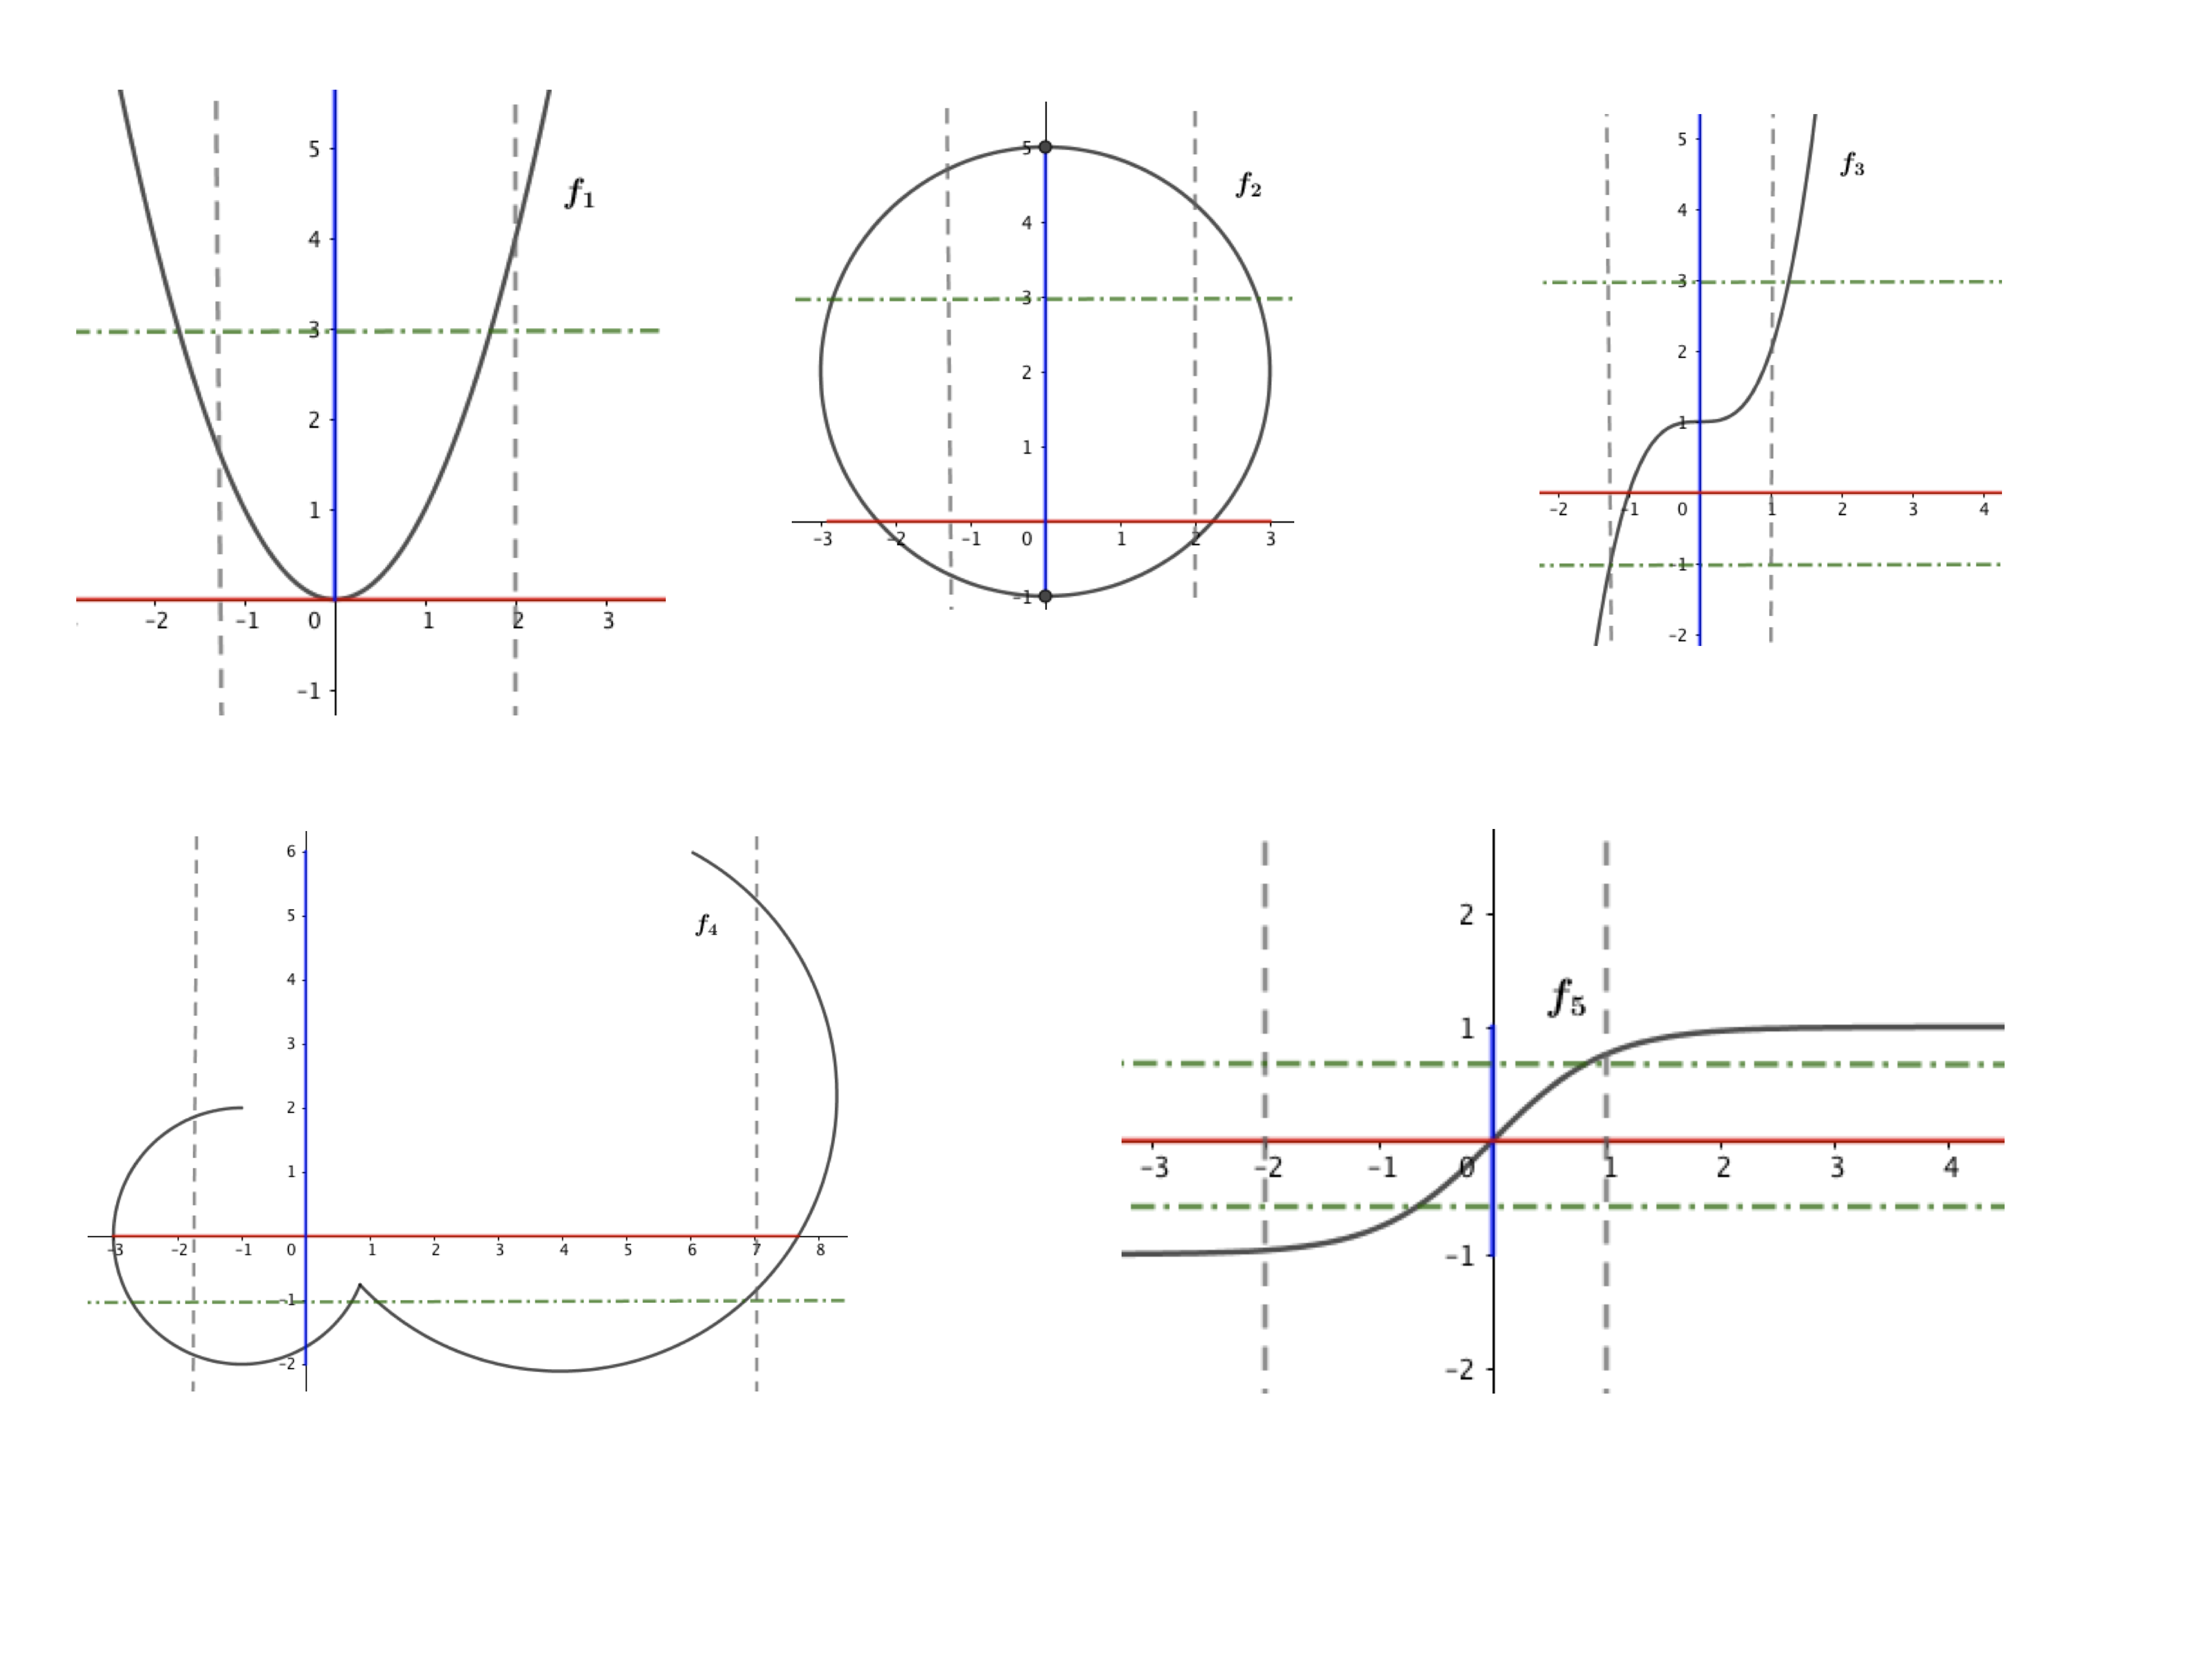
\includegraphics[width=1\textwidth]{imagenes/imagenes02/T02IM21.png}
			
		\end{figure}
		
		\begin{proofw}\renewcommand{\qedsymbol}{$\diamond$}
		En las gráficas aparece en rojo la proyección de la curva sobre $OX$, el dominio; en azul aparece la proyección de la curva sobre $OY$, el recorrido. Usamos la estrategia de la \emph{lí­nea vertical}, en gris, para saber si se trata de una verdadera función matemática y la estrategia de la \emph{lí­nea horizontal}, en verde, pasa averiguar si la función es inyectiva.
		
			 \begin{enumerate}
			 	\item [*] $f_1$: sí­ es función, no inyectiva, Dom=$\mathbb R$, Rec=$[0,\infty[$
			 	\item[*] $f_2$: no función, no inyectiva, 'dom'=$[3,4]$, 'rec'=$[-1,\infty]$
			 	\item [*] $f_3$: sí­ función, sí­ inyectica, Dom=Rec=$\mathbb R$
			 	\item [*] $f_4$: no función, no inyectiva, 'dom'=$[-3,8]$ aprox, 'rec'=$[-2,6]$ aprox.
			 	\item [*] $f_5$: sí­ función, sí­ inyectica, dom=$\mathbb R$, rec=$[-1,1]$
			 \end{enumerate}
		\end{proofw}
		
		
		
		
		\begin{ejre}
			Calcula los dominios (naturales) de las siguientes funciones:
			
		
		
		\begin{multicols}{2} 
		\begin{itemize}
		\item $f_1(x)=\dfrac 1 {1+x^2}$
		\item $f_2(x)=1+\sqrt x$
		\item $f_3(x)=\dfrac 1 {1-\sqrt x}$
		\item $f_4(x)=\sqrt{4-x^2}$
		\item  $f_5(x)=\dfrac 1 {\sqrt{4-x^2}}$
		\item $f_6(x)=\dfrac {1}{x-1} + \dfrac {1}{x+2} $
		\item $f_7(x)=\sqrt {1-x}+\sqrt {x-2}$
		\item $f_8(x)=\sqrt{1-x^2}+\sqrt{x^2-1}$
		\end{itemize}
		\end{multicols}
		

			
		\end{ejre}
		
		\begin{proofw}\renewcommand{\qedsymbol}{$\diamond$}
		
		Soluciones:
		
		\begin{itemize}
			\item [*]$f_1(x)=\dfrac 1 {1+x^2}:\qquad 1+x^2= 0 \to x=\pm \sqrt{-1} \notin \mathbb R \to \quad Dom(f_1)=\mathbb R $ 
			\item [*]$f_2(x)=1+\sqrt x: \qquad x\ge0 \to \quad Dom(f_2)=[0,\infty[=\mathbb R^+_*$
			\item [*]$f_3(x)=\dfrac 1 {1-\sqrt x}: \qquad x\ge 0,\;  $ pero $\; 1-\sqrt x \neq 0; \; \; x\neq \pm 1 \to \quad Dom(f_3)=\mathbb R^+_* \sim \{ \pm 1 \}= [0,1[ \cup ]1,\infty[$
			\item [*]$f_4(x)=\sqrt{4-x^2}: \qquad4-x^2\ge 0;\; 4-x^2=0; \; x=\pm 2$ Construimos una tabla en que estudiamos el signo de $4-x^2$.
			
		
			\begin{table}[H]
			\centering
			\begin{tabular}{|c|c|c|c|c|c|}
				\hline
				 Intervalos & $]-\infty,-2[$  & $-2$ & $]-2,2[$ & $2$ & $]2,\infty[$  \\ \hline
				 $4-x^2$& $-$ & 0 & + & 0 & $-$\\ \hline
			\end{tabular}
			\end{table}
			Luego, $Dom(f_4)=[-2,2]$
		
			\item[*]$f_5(x)=\dfrac 1 {\sqrt{4-x^2}}: \qquad $Ahora, $4-x^2>0$, no vale la opción $4-x^2=0$ porque producirí­a un cero en el denominador, por lo que, con la misma tabla anterior, $Dom(f_5)=]-2,2[$
			\item[*]$f_6(x)=\dfrac {1}{x-1} + \dfrac {1}{x+2}: \qquad D_1 \left( \frac {1}{x-1} \right)=\mathbb R \sim \{1\}; \quad D_2 \left( \frac {1}{x+2} \right)=\mathbb R \sim \{-2\} \to Dom(f_5)=D_1 \cap D_2 = \mathbb R \sim \{ -2,1 \}$
			
			
			\item[*] $f_7(x)=\sqrt{1-x}+\sqrt{x+2}: \qquad D_1: 1-x\ge 0 \to x\le 1:\; ]-\infty, 1]; \qquad D2: x-2\ge 0 \to x\ge 2: \; [2, \infty[ \quad \Rightarrow    \quad D(f_7)=D_1 \cap D_2 = \phi$
			
			\item[*]$f_8(x)=\sqrt {1-x^2}+\sqrt {^2-1}:$. Tanto $1-x^2$ como $x^2-1$ son $0$ cuando $x=\pm1$. Estudiamos los signos en la siguiente tabla:
			
			\begin{table}[H]
			\centering
			\begin{tabular}{|c|c|c|c|c|c|}
			\hline
 				Intervalos & $]-\infty,-1[$  & $-1$ & $]-1,1[$ & $1$ & $]1,\infty[$ \\ \hline
 				$1-x^2$ & $-$ & $0$ & $+$ & $0$  & $-$ \\ \hline
 				$x^2-1$ & $+$  & $0$  & $-$ & $0$  & $+$  \\ \hline
			\end{tabular}
			\end{table}
			
			Como $D_1=D(\sqrt{1-x^2})=]-\infty,-1]\cup [1,\infty]$, y $D_2=D(\sqrt{x^2-1})=[-1,1]$, entonces $Dom(f_8)=D_1 \cap D_2= \{ -1,1 \}$
			
			
		\end{itemize}
			
		\end{proofw}

		
		
		
		\begin{ejre} Dadas las funciones: $f(x)=x^2+1;\; (\forall x\ge0) \quad g(x)=\dfrac {3}{x-2}; \quad h(x)= \sqrt{x-3}$, inyectivas todas ellas en sus dominios de definición, calcula: 
		
		$g\cdot g;\quad g\circ g; \quad f\circ g; \quad g\circ f; \quad f^{-1}; \quad g^{-1}; \quad h^{-1}; \quad  f\circ f^{-1}; \quad (g \circ f)^{-1}; \quad f^{-1} \circ g^{-1} $ 
		
		Dominios y recorridos de todas ellas.
		
		\end{ejre}
		
		\begin{proofw}\renewcommand{\qedsymbol}{$\diamond$}
			
		Soluciones:
			
		\begin{itemize}
			
			
			\item [*] $g\cdot g \to g(x)\cdot g(x)= \dfrac {3}{x-2} \cdot \dfrac {3}{x-2} = \dfrac {9}{(x-2)^2}$
			\item [*] $g\circ g \to g(g(x))=g\left( \dfrac {3}{x-2} \right)=\dfrac {3}{\dfrac {3}{x-2}-2}=\dfrac {3x-6}{7-2x}$
			\item [*] $f\circ g \to f(g(x))=f \left( \dfrac {3}{x-2}  \right) = \left( \dfrac {3}{x-2}  \right)^2 +1 = \dfrac {x^4-4x+13}{x^2-4x+4}$
			
			\item [*] $ g\circ f \to g (f(x))=g(x^2+1)=\dfrac {3}{(x^2+1)-2} = \dfrac {3}{x^2-1} \quad  $ (Nótese que $g\circ f \neq f\circ g$)
			
			\item [*] $f^{-1} \to   y=x^2+1; x\leftrightarrow y: \; x=y^2+1; \; y^2=x-1; \; y=+\sqrt{x-1} \to f^{-1}(x)=+\sqrt{x-1}$
			\item [*] $g^{-1} \to  y=\dfrac {3}{x-2}; x\leftrightarrow y: \; x=\dfrac {3}{y-2}; \; x(y-2)=3; \; y=\dfrac {2x+3}{x} \to g^{-1}(x)=y=\dfrac {2x+3}{x}$
			\item [*] $h^{-1} \to y=\sqrt{x-3}; x\leftrightarrow y: \; x=\sqrt{y-3} ; \; x^2=y-3; y=x^2+3 \to h^{-1}(x)=x^2+3 $
			\item [*] $ f \left(f^{-1}(x) \right) =f (\sqrt {x-1})=(\sqrt{x-1})^2+1=x=I(x) \quad$ (Nótese que $f\circ f^{-1}=I$)
			\item [*] $ (g \circ f )^{-1} \to (g\circ f)(x)= \dfrac {3}{x^2-1}=y ; \; x\leftrightarrow y: \; \dfrac {3}{y^2-1}=x; \; y^2=\dfrac {3+x}{x}; \; y= \sqrt {\dfrac {3+x}{x}} \to  (g \circ f )^{-1}(x)=\sqrt {\dfrac {3+x}{x}}$
			\item [*] $f^{-1} \circ g^{-1} \to f^{-1} \left( g^{-1}  \right)(x)= f^{-1} \left( \dfrac {2x+3}{x} \right) = \sqrt{\left( \dfrac {2x+3}{x} \right)-1}= \sqrt{\dfrac {x+3}{x}} \to$
			
			 	$\left( f^{-1} \circ g^{-1} \right)(x)=\sqrt{\dfrac {x+3}{x}}\quad $ ( Nótese $\;(g \circ f )^{-1} =  f^{-1} \circ g^{-1} \; $ )
			 	\item [*] $Dom(f)=\mathbb R^+; \quad Rec(f)=Dom(f^{-1})=[1, \infty[; \quad Dom(g)=\mathbb R \sim \{2\}; \quad Rec(g)=Dom(g^{-1})=\mathbb R \sim \{0\}; \quad Dom(h)=[3,\infty[; \quad Rec(h)=Dom(h^{-1})=\mathbb R^+ \; $(por la zona de inyectividad de $h(x)=+\sqrt{x-3}$)
		\end{itemize}
			
		\end{proofw}
		
		
		
		\begin{ejre}
		Calcula la inversa de las funciones: $\quad f(x)=\arcsin (x^2-1); \qquad  g(x)=\ln (x^2+1)$
		\end{ejre}
		
		\begin{proofw}\renewcommand{\qedsymbol}{$\diamond$}
			
		Soluciones:
			
		\begin{itemize}
		\item[*] $y=\arcsin (x^2-1): \; x\leftrightarrow y: \; x=\arcsin (y^2-1); \; \sin x= \sin [\arcsin (y^2-1)]=y^2-1; \; y^2=\sin x +1; \; y=\sqrt{\sin x + 1} \; \to \; f^{-1}(x)=\sqrt{\sin x + 1}$	
		
		\item[*] $y=\ln (x^2+1): \; x\leftrightarrow y: \; x=\ln(y^2+1); \; e^x=e^{\ln (y^2+1)}=y^2+1; \; y^2=e^x-1; \; y=\sqrt{e^x-1} \; \to \; g^{-1}(x)= \sqrt{e^x-1}$
		\end{itemize}

		\end{proofw}
		
		
		
		
		
		\begin{ejre} Define como función a trozos: 
		\label{ejre:rompe-trozos}
			
			\begin{multicols}{2} 
			\begin{itemize}
			\item $f_1(x)=|4-x|$
			\item $f_2(x)=|-x^2-2x+3|$
			\item $f_3(x)=|\ln x|$
			\item $f_4(x)=|x|+x$
			\item $f_5(x)=|x+1|-|x-3|$
			\item $f_6(x)=|2x-4|-2|x-1|$
			\item $f_7(x)=\left| \dfrac {x^2-4}{x+1} \right|$
			\item $f_8(x)=\dfrac {|x+3|}{1+|x|}$
			\end{itemize}
			\end{multicols}
			\end{ejre}
		
		\begin{proofw}\renewcommand{\qedsymbol}{$\diamond$}
		
		Soluciones:
		
		
		\begin{itemize}
			\item [*] $f_1(x)=|4-x| \to 4-x=0;\; x=4$
			
			\begin{multicols}{2} 
			
			\begin{table}[H]
			\centering
			\begin{tabular}{|c|c|c|c|}
			\hline
			Intervalos & $]-\infty,4[$ & $4$ & $]4,\infty[$ \\ \hline
			$4-x$ & $+$ & $0$ & $-$ \\ \hline
		\end{tabular}
		\end{table}
		
		\begin{equation*}
		f_1(x)=
		\begin{cases} 
		\;\;  4-x &\mbox{if } x \le 4 \\ 
		\; x-4 & \mbox{if } x >4 
		\end{cases}
		\end{equation*}
		
		\end{multicols}
		
		\item [*] $f_2(x)=|-x^2-2x+3| \to -x^2-2x+3=0; \; x=-3, x=1 $
				\begin{table}[H]
				%\centering
				\begin{tabular}{|c|c|c|c|}
				\hline
				Intervalos & $]-\infty, -3[$ & $[-3,1[$ & $[1, \infty[$ \\ \hline
				$-(x-1)(x+3)$ & $-$ &  $+$ & $-$ \\ \hline	
				\end{tabular}
				\end{table}
			
			\begin{equation*}
				f_2(x)=
				\begin{cases} 
				\;  x^2+2x-3 &\mbox{si } x \le -3 \\ 
				\; -x^2-2x+3 &\mbox{si } -3\le x \le 1 \\
				\;  x^2+2x-3 &\mbox{si } x>1
				\end{cases}
			\end{equation*}
				
			
			
		\item[*] $f_3(x)=|\ln x| \to \ln x=0; \; x=e^0=1 \qquad \ln x:[0,\infty[ \to  \mathbb R[$
		
			\begin{multicols}{2} 
			
				\begin{table}[H]
					\centering
					\begin{tabular}{|c|c|c|c|}
					\hline
					Intervalos & $]0, 1[$ & $1$ & $]1, \infty[$ \\ \hline
					$\ln x$ & $-$ &  $0$ & $+$ \\ \hline	
					\end{tabular}
				\end{table}
			
				\begin{equation*}
					f_3(x)=
					\begin{cases} 
					\;  -\ln x &\mbox{si } 0<x<1 \\ 
					\; \ln x &\mbox{si } x\ge 1 
					\end{cases}
				\end{equation*}
				
			\end{multicols}
			
		\item [*] $f_4(x)=|x|+x$
			
				\begin{equation*}
					f_4(x)=
					\begin{cases} 
					\;  -x+x\; = \; 0 &\mbox{si } x<0 \\ 
					\; x+x\; = \; 2x&\mbox{si } x\ge 0 
					\end{cases}
				\end{equation*}
		
		\item [*] $f_5(x)=|x+1|-|x-3| \to x+1=0;x=-1; \; x-3=0; x=3$
		 
			\begin{multicols}{2} 
			
				\begin{table}[H]
					\centering
					\begin{tabular}{|c|c|c|c|}
					\hline
					Intervalos & $]-\infty, -1[$ & $[-1,3]$ & $]3, \infty[$ \\ \hline
					$x+1$ & $-$ &  $+$ & $+$ \\ \hline	
					$|x+1|$ & $-x-1$ & $x+1$ & $x+1$ \\ \hline
					$x-3$ & $-$ & $-$ & $+$ \\ \hline
					$|x-3|$ & $-x+3$ & $x-3$ & $x-3$ \\ \hline
					$f_5$ & $-4$ & $2x-2$ & $4$ \\ \hline
					\end{tabular}
				\end{table}
			
				\begin{equation*}
					f_3(x)=
					\begin{cases} 
					\;  -4 x &\mbox{si } x<1 \\ 
					\; 2x+2 &\mbox{si } -º\le x \le 3 \\
					\;    4   & \mbox{si } x>3
					\end{cases}
				\end{equation*}
				
			\end{multicols}
			
		\item[*] $f_6(x)=|2x-4|-2|x-1| \to 2x-4=0; x=2; \; x-1=0; x=1$ 
		
			\begin{multicols}{2} 
			
				\begin{table}[H]
					\centering
					\begin{tabular}{|c|c|c|c|}
					\hline
					Intervalos & $]-\infty, 1[$ & $[1,2]$ & $]2, \infty[$ \\ \hline
					$2x-4$ & $-$ &  $-$ & $+$ \\ \hline	
					  $|2x-4|$ & $-2x+4$  & $-2x+4$  & $2x-4$     \\ \hline
					 $x-1$  & $-$  & $+$  & $+$   \\ \hline
					 $-2|x-1|$  & $2x-2$  & $-2x+2$  & $-2x+2$   \\ \hline
					 $f_6$  & $2$  & $-4x+6$  & $-2$   \\ \hline 
					\end{tabular}
				\end{table}
			
				\begin{equation*}
					f_6(x)=
					\begin{cases} 
					\;  2 &\mbox{si } 0<1 \\ 
					\; -4x+6 &\mbox{si } 1\le x \le 2 \\ 
					\; -2 2 &\mbox{si } x>2
					\end{cases}
				\end{equation*}
				
			\end{multicols}
		
		\item[*] $f_7(x)=\left| \dfrac {x^2-4}{x+1} \right| \to x^2-4=0; x=\pm 2; ; x+1=0; x\neq -1$ 
		
			
			    
				\begin{table}[H]
					\centering
					\begin{tabular}{|c|c|c|c|c|}
					\hline
					Intervalos & $]-\infty, -2]$ & $]-2,-1[$&$]-1,2[$ & $[2, \infty[$ \\ \hline
					$x^2-4$ & $+$ &  $-$ & $-$ & $+$\\ \hline	
					$|x^2-4|$ & $x^2-4$ &  $-x^2+4$ & $-x^2+4$ & $x^2-4$\\ \hline
					$x+1$ & $-$ &  $-$ & $+$ & $+$\\ \hline
					$x+1$ & $-x-1$ &  $-x-1$ & $x+1$ & $x+1$\\ \hline
					$f_7$ & $-\dfrac{x^2-4}{x+1}$ &  $\dfrac{x^2-4}{x+1}$ & $-\dfrac{x^2-4}{x+1}$ & $\dfrac{x^2-4}{x+1}$\\ \hline
					
					\end{tabular}
				\end{table} 
			
				\begin{equation*}
					f_7(x)=
					\begin{cases} 
					\;  -\dfrac{x^2-4}{x+1} &\mbox{si } x\le -2 \\ 
					\; \dfrac{x^2-4}{x+1} &\mbox{si } -2<x< -1 \\
					\;  -\dfrac{x^2-4}{x+1} &\mbox{si } -1<x<2 \\ 
					\; \dfrac{x^2-4}{x+1} &\mbox{si } x\ge 2
					\end{cases}
				\end{equation*}
				
			\item[*] $f_8(x)=\dfrac {|x+3|}{1+|x|} \to x+3=0; x=-3; ; x=0$
		
				\begin{multicols}{2} 
			
				\begin{table}[H]
					\centering
					\begin{tabular}{|c|c|c|c|}
					\hline
					Intervalos & $]-\infty, -3[$ & $[-3,0]$ & $]0, \infty[$ \\ \hline
					$x+3$ & $-$ &  $+$ & $+$ \\ \hline	
					$x$   &  $-$  &  $-$  &  $+$ \\ \hline
					$f_8$   &  $\dfrac {-x-3}{1-x}$  &  $\dfrac {x+3}{1-x}$  &  $\dfrac {x+3}{1+x}$ \\ \hline
					\end{tabular}
				\end{table}
			
				\begin{equation*}
					f_8(x)=
					\begin{cases} 
					\;  \dfrac {x+3}{x-1} &\mbox{si } x<-3 \\ 
					\; \dfrac {x+3}{1-x} &\mbox{si } -3\le x \le 0 \\
					\; \dfrac {x+3}{1+x} & \mbox{si } x>0 
					\end{cases}
				\end{equation*}
				
				\end{multicols}
		
		
		\end{itemize}
		
			
		\end{proofw}
		
		
		\begin{ejre}
		Estudia la paridad de las siguientes funciones:
		
		\begin{multicols}{2} 
			\begin{itemize}
			\item $f_1(x)=x^2+1$
			\item $f_2(x)=x^5-x^3-x$
			\item $f_3(x=1-\cos x$
			\item $f_4(x)=\dfrac {x^4+1}{x^3-2x}$
			\item $f_5(x)=1-\sin x$
			\item $f_6(x)=x+\cos x$
			\item $f_7(x)=\sqrt{x^4-1}$
			\item $f_8(x)=\dfrac {x}{x^3-1}$
			\item $f_9(x)=e^{|x|}$
			\item $f_{10}(x)=\dfrac {|x|}{x^2-2x}$
			\item $f_{11}(x)=\arcsin x$
			\end{itemize}
			\end{multicols}
		
		\end{ejre}
		
		\begin{proofw}\renewcommand{\qedsymbol}{$\diamond$}	

		Soluciones:
		
		\begin{itemize}
		
			\item [*] $f_1(x)=x^2+1 \to f_1(-x)=(-x)^2+1=x^2+1=f_1(x) \quad $ PAR
			\item [*]  $f_2(x)=x^5-x^3-x \to f_2(-x)=(-x)^5-(-x)^3-(-x)=-x^5+x^3+x=-f_2(x) \quad $ IMPAR
			\item [*]  $f_3(x)=1-\cos x \to f_3(-x)=1-\cos (-x)=1-\cos x=f_3(x) \quad $ PAR
			\item [*]  $f_4(x)=\dfrac {x^4+1}{x^3-2x} \to f_4(-x)=\dfrac {(-x)^4+1}{(-x)^3-2(-x)}=\dfrac {x^4+1}{-x^3+2x}=-\dfrac {x^4+1}{x^3-2x}=-f_4(x) \quad $ IMPAR 
			\item [*]  $f_5(x)=1-\sin x \to  f_5(-x)=1-\sin (-x)=f_5(x)=1+\sin x \quad $ Sin paridad
			\item [*]  $f_6(x)=x+\cos x \to f_6(-x)=-x+\cos (-x)=-x+\cos x \quad  $ Sin paridad
			\item [*]  $f_7(x)=\sqrt{x^4-1} \to f_7(-x)=\sqrt{(-x)^4-1}=\sqrt{x^4-1}=f_7(x) \quad  $ PAR
			\item [*]  $f_8(x)=\dfrac {x}{x^3-1} \to f_8(-x)=\dfrac {-x}{(-x)^3-1}=\dfrac {-x}{-x^3-1}=\dfrac {x}{x^3+1} \quad $ Sin paridad
			\item [*]  $f_9(x)=e^{|x|} \to f_9(-x)=e^{|-x|}=e^{|x|}=f_9(x) \quad $ PAR
			\item [*]  $f_{10}(x)=\dfrac {|x|}{x^2-2x} \to f_{10}(-x)=\dfrac {|-x|}{(-x)^2-2(-x)}=\dfrac {|x|}{x^2+2x} \quad $ Sin paridad
			\item [*]  $f_{11}(x)=\arcsin x \to f_{11}(-x)=\arcsin (-x)=-\arcsin x = -f_{11}(x) \quad $ IMPAR
			
		\end{itemize}

		
		\end{proofw}
		
		\begin{ejre}
		Intenta dibujar la función: 
		\begin{equation*}
		f(x)=
		\begin{cases} 
		\;\;  x &\mbox{if } x \in \mathbb{Q} \\ 
		\; 0 & \mbox{if } x \in \mathbb{R} \sim \mathbb{Q} 
		\end{cases}
		\end{equation*}
		?`Observas algo interesante?
		\end{ejre}
		
		\begin{proofw}\renewcommand{\qedsymbol}{$\diamond$}
		
		Solución: \scriptsize{Solo `continua' en cero.}
		
			\begin{figure}[H]
			\centering
			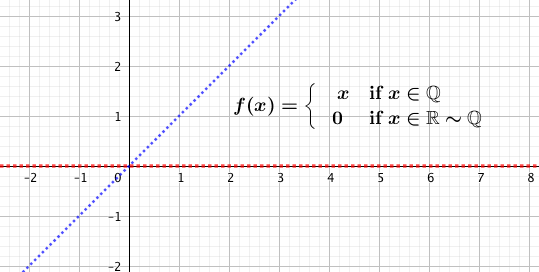
\includegraphics[width=0.5\textwidth]{imagenes/imagenes02/T02IM23.png}
			%\caption{Función solo continua en cero.}
			\end{figure}
			
		\end{proofw}
		
		\subsection{Ejercicios Propuestos}	
		
		
		\begin{enumerate}[1).-  ]
		\item A partir de la función representada en la siguiente gráfica, $f(x)$, estudia si es inyectiva, su dominio, su recorrido y, a partir de ella, representa:
		
			$f(x)+3; \quad f(x)-1; \quad f(x-2); \quad f(x+1); \quad 2f(x); \quad f(-x); \quad -f(x); \quad -f(-x)$
		
			\begin{figure}[H]
			\centering
			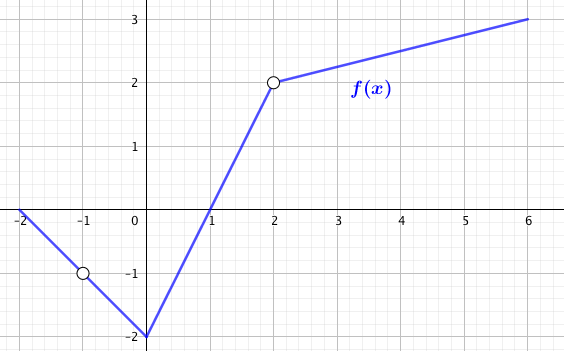
\includegraphics[width=0.6\textwidth]{imagenes/imagenes02/T02IM22.png}	
			\end{figure}
		
		
		\rightline{\textcolor{gris}{Solución:  \tiny{Sí­ inyectiva, $Dom(f)=[-2,-1[\cup ]-1,2[ \cup ]2,6]$; $\; Rec(f)=[-2,2[ \cup ]2,3]$}}}
		
		\item La \emph{función de Heaviside} es muy usada en ciencia, se define por:
		
			\begin{equation*}
			H(x)=
			\begin{cases} 
			\;\;  1 &\mbox{if } x \ge 0 \\ 
			\; 0 & \mbox{if } x<0 
			\end{cases}
			\end{equation*}
	
		Dibuja la función de Haeviside y también: $H(x)-2;\quad H(x-2); \quad -H(x-2)-2$
		
		\item Calcula el dominio de las siguientes funciones:
		
		\begin{multicols}{2} 
		\begin{enumerate}[a.]
		\item $f(x)=\ln{4-\sqrt x}$
		\item $f(x)=\dfrac 1 {\tan x}$
		\item $f(x)=\dfrac 1 {\sqrt {\tan^2 x - 1}}$
		\item $f(x)=\dfrac {2}{1-\cos x}$
		\item $f(x)=\dfrac {1}{\sin x - \frac 1 2}$
		\end{enumerate}
		\end{multicols}

		
		\rightline{\textcolor{gris}{Solución:  $D_a=[0,16[;\quad D_b=\mathbb R \sim \{ k\pi, (2k+1)	pi /2\};\; \forall k \in \mathbb Z$}}
		\rightline{\textcolor{gris}{ $D_c=[-\frac {\pi}{2}+k\pi, -\frac {\pi}{4}+k\pi[ \cup ] \frac {\pi}{4}+k\pi , \frac {\pi}{2} +k\pi  [ ; \; \forall k\in \mathbb Z$}}
		\rightline{\textcolor{gris}{ $D_d=\mathbb R \sim \{2k\pi; \; \forall k \in \mathbb Z \} \quad D_e= \mathbb R \sim \{ \frac {\pi}{6}+2k\pi, \; \frac {5\pi}{6}+2k\pi ;\;\forall k \in \mathbb Z \}$ }}
		
		
		\item Dadas las funciones: $f(x)=\sin x ; \quad g(x)=\pi x$, evalúa las expresiones siguientes:
		
		 	\begin{multicols}{3} 
			\begin{enumerate}[a.]
				\item $f(g(2))$
				\item $f(g(1/2))$
				\item $g(f(0))$
				\item $g(f(\pi /4))$
				\item $f(g(x))$
				\item $g(f(x))$
			\end{enumerate}
			\end{multicols}
			
			\rightline{\textcolor{gris}{Solución: a)$0$; b)$1$; c)$0$ }}
			\rightline{\textcolor{gris}{Solución: d)$\sqrt 2 \pi /2$;  e) $\sin \pi x$;  f) $\pi \sin x$ }}
		
		 
		 \item para los siguientes pares de funciones, calcula $f\circ f$, $g \circ f$ y los dominios de ambas composiciones.
		 
		 	\begin{multicols}{2}
		 	\begin{enumerate}[a. ]
		 		\item $f(x)=\frac 3 x \; ;\quad g(x)=x^2-1$
		 		\item $f(x)= \frac 1 x\; ; \quad g(x)=\sqrt{x+2}$
		 	\end{enumerate}	
		 	\end{multicols}
			
			\rightline{\textcolor{gris}{Solución: a) $D(f\circ g)=\mathbb R \sim \{ -1,1\}; \quad D(g\circ f)=\mathbb R \sim \{ 0\}$ }}
			\rightline{\textcolor{gris}{Solución: b) $D(f\circ g)=]-2, \infty[; \quad D(g\circ f)=]-\infty, -1/2] \cup ]0, \infty[$  }}

		 \item Determina $f\circ g$ siendo las funciones $f$ y $g$ las definidas definidas por: 
		 
		 	\begin{equation*}
			f(x)=
			\begin{cases} 
			\;\;  x+3 &\mbox{if } x<0 \\ 
			\; 2x^2+3 & \mbox{if } x\ge 0 
			\end{cases}
			\qquad g(x)=x+1
			\end{equation*}
		 
		 \item Calcula la inversa de la función $f(x)=\sqrt{\dfrac{x-1}{x+1}}$
		
		 \rightline{\textcolor{gris}{Solución: $y=\frac {x^2+1}{x^2-1} $}}

		

		
		\item Si $f(2^x)=x^2$, calcula $f(16)$
		 
		\rightline{\textcolor{gris}{Solución: 16}}
		
		
		
		\item Si $f(2x-1)=x$, calcula $f(2)$
		 
		\rightline{\textcolor{gris}{Solución: $3/2$}}
		
		
		
		\item Si $f(x+4)=2x+3$, calcula $f(f(f(f(x))))$
		 
		\rightline{\textcolor{gris}{Solución: $3x-155$}}
		
		
		
		\item Si $f(x)=\dfrac {x}{x-1}, \; x\neq 1$, calcula $(f\circ f \circ \cdots \circ f)_{9\mbox{ veces }}(x)$
		 
		\rightline{\textcolor{gris}{Solución: f(x)}}
		
		
		
		\item Si $f(x)=\dfrac {x+1}{x-1}$, calcula $f(f(f(f(2020))))$
		 
		\rightline{\textcolor{gris}{Solución: 2020 }}
		
		\item Si $f(f(f(f(x))))=16x+15$, calcula $f(7)$
		 
		\rightline{\textcolor{gris}{Solución: ayuda, considera $f(x)=ax+b$}}
		
		\item Sea $f(x)=x^3+3$, $g(f(x))=x,\; \forall x$, calcula $g(30)$
		 
		\rightline{\textcolor{gris}{Solución: 3}}
		
		\item $\divideontimes$. Sea $f(x)$ una función real de variable real tal que $f(x-5)=f(x+5)$ y se sabe que tiene 5 raí­ces reales distintas \scriptsize{(raí­z de $f(x)$ es cada una de las soluciones de la ecuación $f(x)=0$)} \normalsize{Calcula la suma de todas ellas.}
		 
		\rightline{\textcolor{gris}{Solución:25 }}
		
		
			
		\end{enumerate}
		

			



